\chapter[Gestión, planificación y desarrollo del software]{Gestión, planificación y desarrollo del proyecto de software}
Ya hemos introducido las bases del \textit{testing}, de la computación cuántica y de las pruebas de mutación aplicada a la misma. Estamos en disposición de hablar del \textit{software} realizado y que trabaja sobre todos estos conocimientos.

\section{Gestión del proyecto}

En primer lugar vamos a tratar acerca de todo el proceso de gestión del proyecto, desde la organización como equipo, hasta herramientas y \textit{software} utilizado para el desarrollar el código y la memoria.

\subsection{Gestión de equipo}

La gestión del equipo es sencilla, en principio los dos miembros del grupo contamos con el mismo poder para la toma de decisiones y por tanto, dichas decisiones han de tomarse de manera consensuada. Si bien es cierto que, según la actividad, alguno de los miembros puede estar más involucrado en ella y es razonable que sus argumentos tenga un mayor peso.

Además, en caso de decisiones clave siempre teníamos una segunda opinión, correspondiente a nuestro tutor, que por tanto ha formado parte también de la toma de las mismas. Hemos tratado de involucrarnos por igual en todas las fases y tareas del TFG con, tal vez, algunas excepciones. Veremos a continuación de forma detallada la contribución de cada uno al trabajo.

\subsection{Contribución al proyecto de Luis Aguirre}
% Al menos dos páginas

\subsection{Contribución al proyecto de Javier Pellejero}
% Al menos dos páginas

\subsection{Gestión de configuración}

Hablemos ahora de todas las herramientas y elementos de \textit{software} utilizados para el proyecto. Empezando por esta memoria, al estar realizada en \LaTeX, hemos necesitado programas para su edición y compilación. Ambos componentes del grupo hemos utilizado como distribución \textit{MiKTeX}, mientras que como editor hemos usado \textit{Texmaker}.

En cuanto al \textit{software}, el grueso del programa está realizado en \textit{Java} y es utilizado como gestor y editor del mismo la plataforma \textit{Eclipse} usando como herramienta de desarrollo la octava versión \textit{Java SE Development Kit} (JDK) de \textit{Oracle}.

El programa principal debe realizar una serie de test sobre los lenguajes de computación cuántica \qsh\ y \textit{Qiskit}. En el caso del primero, permite ser llamado desde \csh\ y {Python}, siendo más común utilizar el primero. En el caso del segundo, más que un lenguaje en sí mismo, es un marco de trabajo que engloba varias librerías que se ejecutan sobre \textit{Python}. Se opta por dejar \csh\ de lado, puesto que \textit{Python} es el lenguaje en común de ambos, y nuestro programa principal, mediante una llamada a sistema, ejecute un programa en dicho lenguaje.

Este programa cambia con cada ejecución y es el programa en \textit{Java} principal quien debe escribirlo. Sin embargo, se han de escribir archivos adicionales en \textit{Python} que contienen funciones útiles y siempre necesarias y para ello se emplea un programa de edición sencillo como \textit{Notepad++}, además de \textit{Jupyter Notebook}, usando la distribución \textit{Anaconda}, para verificar que nuestras funciones escritas tanto por nosotros como por el programa funcionan correctamente.

Para el correcto funcionamiento del programa en su conjunto, se necesitan una serie de requisitos.

\begin{itemize}
\item Una máquina virtual capaz de ejecutar \textit{Java} como \textit{Java Runtime Environment} (JRE).
\item \textit{Python} 2 o 3. (Se recomienda \textit{Python} 3).
\item La librería de \textit{Python} \textit{func-timeout} de Tim Savannah bajo licencia LGPLv3 accesible en \textbf{https://github.com/kata198/func\_timeout/blob/master/LICENSE}. Se adjunta en el repositorio del proyecto.
\item \qsh\ (sólo si se realizaran test con este lenguaje cuántico).
\item \textit{Qiskit} (sólo si se realizaran test con este lenguaje cuántico).
\end{itemize}

En cuanto a la organización y distribución de nuestro código, hemos elegido \textit{Github}. Además de ser un excelente gestor de versiones, tiene el programa (para el sistema operativo\textit{Windows}) \textit{Github Desktop}, una interfaz sencilla para subir y gestionar el código. En el repositorio existen dos carpetas principales en el directorio raíz:

\begin{itemize}
\item \textbf{tex}: que almacena el código \LaTeX.
\item \textbf{src}: que almacena el código, tanto \textit{Java} como \textit{Python}
\end{itemize}

Además existen otras carpetas de menor relevancia con contenidos como ejemplos en los dos lenguajes cuánticos tratados, presentaciones, además de encontrarse en la raíz principal la \textbf{licencia MIT}.

Como veremos, este programa no sólo puede ser realmente utilizado por cualquier interesado en realizar pruebas de mutación sobre programas cuánticos, sino que pueden ser integradas una serie de funcionalidades adicionales en el mismo. Por ello hemos optado por esta licencia, que posiblemente sea la de menor número de restricciones. Cualquiera puede tomar el proyecto y modificarlo, incluso para uso comercial.

\section{Planificación}

La planificación del proyecto puede dividirse en dos aspectos: uno desde el punto de vista temporal que incluye el proceso de investigación, \textit{software} y la realización de la memoria; y otro desde el punto de vista del modelo de proceso elegido para el \textit{software}.

\subsection{Planificación temporal}

Para planificar este Trabajo de Fin de Grado es importante entender que, como alumnos del doble grado en ingeniería informática y matemáticas, debemos realizar un TFG por grado. Nuestra idea inicial es que ambos trabajos estuvieran relacionados y ya en julio contactamos con nuestro tutor y conocíamos el tema de los mismos.

Dejamos constancia de que en el caso del TFG de matemáticas, dichos trabajos eran individuales aunque ambos alumnos tratamos un tema común que es el de introducirnos en la computación cuántica con una sólida base matemática y con alguna pincelada de conocimiento en mecánica cuántica. Además, cada uno introduce un lenguaje de programación cuántico: \qsh\ en el caso de Luis Aguirre y \textit{Qiskit} en el caso de Javier Pellejero.

Por tanto, se puede argumentar que este trabajo tiene sus cimientos en los dos realizados por cada miembro del grupo para el grado de matemáticas. Explicado esto, empezaremos por enumerar una serie de fases de planificación que incluye todos los trabajos.

\begin{enumerate}
\item \textbf{Proceso de investigación}. Puesto que se trata de una serie de conocimientos totalmente nuevos para nosotros y con una complejidad considerada, es importante dotar a esta fase de una duración prolongada. Decidimos establecer como límite para esta fase finales de enero coincidiendo con el fin de exámenes del primer cuatrimestre. En el segundo, ninguno de los integrantes del grupo tiene otras asignaturas, así que hay tiempo suficiente para el resto de fases.
\item \textbf{Desarrollo del \textit{software}}. Una vez familiarizados con la teoría de la computación cuántica y de pruebas de mutación, estamos en condiciones de comenzar nuestro programa. En las siguientes páginas se dará más detalle del mismo. En cuanto al tiempo, estimamos unos dos meses, febrero y marzo, para realizarlo.
\item \textbf{Memorias individuales del TFG del grado de matemáticas}. Por lo comentado anteriormente, es consecuente realizar primero estas memorias pues su contenido sirve de base para desarrollar esta misma. Se estable que el tiempo marcado por el mes de abril es apropiado para realizarla.
\item \textbf{Memoria del TFG del grado en ingeniería informática}. Siguiente tarea a efectuar. Prevista para el mes de mayo.
\item \textbf{Revisión}. Se establece el mes de junio para ultimar memorias, perfección del \textit{software} o cualquier otra tarea que pudiera no estar acabada.
\end{enumerate}

Aclaramos que estas fechas son orientativas. Como veremos a continuación, nuestro modelo de proceso del \textit{software} se asemeja a un \textbf{desarrollo evolutivo ágil}, concretamente al denominado \textbf{\textit{eXtreme Programming}} (XP) y sus principios pueden aplicarse también a toda la planificación anterior. Puesto que el tiempo no parece un problema determinante, no seremos estrictos con las fases anteriormente mencionadas.

\subsection{Modelo de proceso}

Acabamos de comentar el modelo en el que se basa nuestro desarrollo del programa. Creemos poder dar algunos buenos argumentos de por qué es una buena decisión. Al contar con un grupo de tan solo dos integrantes, la comunicación entre ambos es clara, concisa y rápida, no sólo entre nosotros sino también con el tutor (al que podemos asignar el rol de cliente), lo que ayuda a prevenir malentendidos que acaban en errores y problemas difíciles de vaticinar aún con un proceso de desarrollo pesado con una planificación más exhaustiva como el proceso unificado.

Otro factor a tener en cuenta es que, si bien los conceptos sobre los que trata nuestro programa no son elementales, no es excesivamente complejo el hecho de implementarlos. Además, al ser un área de la computación en el que no se ha investigado aún en exceso, puede surgir en cualquier momento la necesidad de cambios o implementar nuevas funcionalidades.

El uso de XP facilita este último hecho, pues intercala continuamente diseño y desarrollo de manera evolutiva e iterativa. En nuestro caso, es muy importante disponer de una versión ejecutable del programa desde el momento que esté desarrollada la primera funcionalidad, lo cual hemos logrado. Para ello, diseñamos una vista, le damos forma mediante código y la ensamblamos con la lógica. Antes de continuar una nueva vista, nos aseguramos que la funcionalidad implementada tiene una correcta actividad para evitar el encadenamiento de errores.

%------- Figura iteración XP
\begin{figure}[!h]
\begin{center}
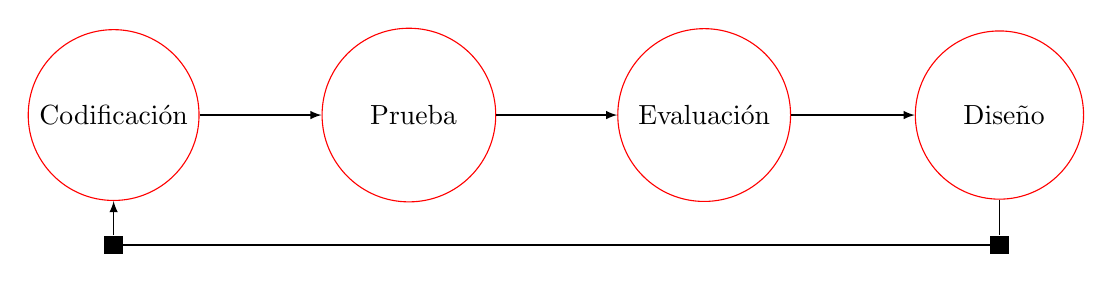
\begin{tikzpicture}[x=1.5cm, y=1.5cm]
	%\fill (-3.2,0) circle (0.1pt)node[anchor=east] {$20$};
	%\fill (3.2,0) circle (0.1pt)node[anchor=west] {$-20$};
    \node[circle,draw=red] (v1) at (-3.75,0) {Codificación};
    \node[circle,draw=red] (v2) at (-1.25,0) {\ \ \ \ Prueba\ \ \ \ };
    \node[circle,draw=red] (v3) at (1.25,0) {\ Evaluación\ \ };
    \node[circle,draw=red] (v4) at (3.75,0) {\ \ \ \ Diseño\ \ \ \ };
    \node[fill=black] (a1) at (-3.75,-1.1) {};
    \node[fill=black] (a2) at (3.75,-1.1) {};
    \draw[color=black, -latex]  (v1) edge (v2);
    \draw[color=black, -latex]  (v2) edge (v3);
    \draw[color=black, -latex]  (v3) edge (v4);
    %\draw[color=black]  (v4) edge (a2);
    %\draw[color=black]  (a2) edge (a1);
    \draw[color=black, -latex]  (a1) edge (v1);
    \draw (v4) -- (a2) -- (a1);
\end{tikzpicture}
\end{center}
\caption{Iteración de etapas en XP.}
\label{fig:fig1}
\end{figure}

En la figura \ref{fig:fig1} podemos observar un diagrama de las etapas estándar de XP. Si bien la primera etapa se corresponde normalmente con la codificación, en nuestro caso siempre lo ha sido el diseño. Así, para cada funcionalidad, se diseña la vista, se implementa la misma, a continuación se desarrolla y enlaza la lógica y por último se prueba. Se itera sobre estas etapas para cada vista y funcionalidad establecidas.

Se sigue así una planificación diseñada prácticamente para cada funcionalidad (planificación incremental) marcándose objetivos a muy corto plazo pero sin perder de vista el objetivo final: completar el programa y su correcto funcionamiento.

Para concluir, hemos tratado de hacer nuestro código lo más adaptable posible, no sólo por el tipo de proceso de desarrollo elegido, sino también para facilitar futuras implementaciones de nuevas funciones para el programa. Esto, sumado a todo lo contado en los anteriores párrafos, justifica que nuestro proceso de desarrollo se ajuste a XP y su correcta elección.

\section{\textit{Mutation Testing for Quantum Computing} (MTQC)}

MTQC son las siglas que dan nombre a nuestro programa. Su principal funcionalidad es la de aplicar pruebas de mutación en distintos lenguajes cuánticos, en nuestro caso \qsh\ y \textit{Qiskit}.

La secuencia de acciones de un usuario en poder de MTQC sería la de generar mutantes del programa deseado, verificar el resultado de los mutantes creados, ejecutar el programa original y los mutantes seleccionados dadas una serie de test y cotejar los resultados para encontrar test satisfactorios e indeseados.

Sobre estas cuatro fases hemos establecido toda nuestra planificación, análisis y diseño del proyecto y es así como vamos a explicar todo el proyecto, tomando estas etapas como estructura de cara al desarrollo.

\subsection{Principales casos de uso}

Los principales casos de uso podemos identificarlos con las fases recientemente nombradas. Podríamos definir algún otro caso como el de elegir un lenguaje cuántico o el de reiniciar el programa, pero el grueso del contenido de MTQC lo recogen estos cuatro:

\begin{itemize}
\item \textbf{Generación de mutantes}. Se trata de la primera acción que el usuario debe realizar. Consta de dos entradas consistentes en dos listas: una del directorio de los archivos de código sobre los que se quiere realizar mutación y otra de los operadores de mutación a aplicar. Arroja como salida una lista de mutantes vinculados al archivo original, el operador aplicado y la línea que sufrió la mutación. En caso de que la fabricación de un mutante arroje un error, se muestra un error por pantalla y se trata de generar el siguiente.

\item \textbf{Visualización de mutantes}. La precondición para que este caso de uso se pueda llevar a cabo es que previamente el usuario haya generado al menos un mutante. Toma como entrada una lista de mutantes con la que el usuario puede interactuar para así poder comparar el contenido de dicho mutante y el archivo original. El objetivo es que el usuario pueda tomar una decisión sobre si el mutante en cuestión es o no un candidato apto para ejecutar un test sobre él.

\item \textbf{Testeo de mutantes}. Se trata del caso de uso principal del programa por importancia, cantidad y calidad del código asociado al mismo. Es necesario verificar la precondición de haber generado al menos un mutante para realizar cualquier acción sobre el mismo. Enumeraremos las entradas.
	\begin{itemize}
	\item Un archivo de código del lenguaje cuántico elegido en ese momento.
	\item Una función contenida en el archivo anterior.
	\item Una lista de todos los mutantes deseados para ejecución generados a partir de dicho archivo.
	\item Un tipo de test a aplicar (determinista o probabilista).
	\item Un conjunto de test.
	\end{itemize}
	
La salida arrojará un conjunto de objetos que gestione los resultados arrojados tras la ejecución de los test y sobre la muerte o no de los mutantes.

\item \textbf{Visualización de los resultados de los test}. Por último, tenemos la opción de que el usuario vea los resultados que los test han arrojado al ser ejecutados sobre la función original y los mutantes, determinar cuántos de ellos han sido matados y la eficacias de dichos test. La precondición indispensable para llevar a cabo esta visualización es haber llevado a cabo las acciones mencionadas en el anterior caso de uso. Toma como entrada un conjunto de objetos que gestionan los resultados de los test y muestra la información correspondiente, previo tratamiento, por pantalla. En el caso de que el test realizado haya sido de tipo probabilista, tomará también como entrada un porcentaje de confianza.
\end{itemize}

\subsection{Diseño}
% Introducción, patrones introducidos (MVC,Observer, Factory)

% Estructura de paquetes

% Explicación de subsistemas + ¿Diagrama de clases? Si es así, ¿en apéndice?

\section{Implementaciones futuras}